% Options for packages loaded elsewhere
\PassOptionsToPackage{unicode}{hyperref}
\PassOptionsToPackage{hyphens}{url}
%
\documentclass[
]{article}
\usepackage{lmodern}
\usepackage{amssymb,amsmath}
\usepackage{ifxetex,ifluatex}
\ifnum 0\ifxetex 1\fi\ifluatex 1\fi=0 % if pdftex
  \usepackage[T1]{fontenc}
  \usepackage[utf8]{inputenc}
  \usepackage{textcomp} % provide euro and other symbols
\else % if luatex or xetex
  \usepackage{unicode-math}
  \defaultfontfeatures{Scale=MatchLowercase}
  \defaultfontfeatures[\rmfamily]{Ligatures=TeX,Scale=1}
\fi
% Use upquote if available, for straight quotes in verbatim environments
\IfFileExists{upquote.sty}{\usepackage{upquote}}{}
\IfFileExists{microtype.sty}{% use microtype if available
  \usepackage[]{microtype}
  \UseMicrotypeSet[protrusion]{basicmath} % disable protrusion for tt fonts
}{}
\makeatletter
\@ifundefined{KOMAClassName}{% if non-KOMA class
  \IfFileExists{parskip.sty}{%
    \usepackage{parskip}
  }{% else
    \setlength{\parindent}{0pt}
    \setlength{\parskip}{6pt plus 2pt minus 1pt}}
}{% if KOMA class
  \KOMAoptions{parskip=half}}
\makeatother
\usepackage{xcolor}
\IfFileExists{xurl.sty}{\usepackage{xurl}}{} % add URL line breaks if available
\IfFileExists{bookmark.sty}{\usepackage{bookmark}}{\usepackage{hyperref}}
\hypersetup{
  pdftitle={Canonisation},
  hidelinks,
  pdfcreator={LaTeX via pandoc}}
\urlstyle{same} % disable monospaced font for URLs
\usepackage{graphicx,grffile}
\makeatletter
\def\maxwidth{\ifdim\Gin@nat@width>\linewidth\linewidth\else\Gin@nat@width\fi}
\def\maxheight{\ifdim\Gin@nat@height>\textheight\textheight\else\Gin@nat@height\fi}
\makeatother
% Scale images if necessary, so that they will not overflow the page
% margins by default, and it is still possible to overwrite the defaults
% using explicit options in \includegraphics[width, height, ...]{}
\setkeys{Gin}{width=\maxwidth,height=\maxheight,keepaspectratio}
% Set default figure placement to htbp
\makeatletter
\def\fps@figure{htbp}
\makeatother
\setlength{\emergencystretch}{3em} % prevent overfull lines
\providecommand{\tightlist}{%
  \setlength{\itemsep}{0pt}\setlength{\parskip}{0pt}}
\setcounter{secnumdepth}{-\maxdimen} % remove section numbering
\usepackage{minted}

\title{Canonisation}
\date{}

\begin{document}
\maketitle

\hypertarget{abstract}{%
\subsection{Abstract}\label{abstract}}

It's useful to be able to evaluate the sub-expressions of an expression
in any order. If tree expressions did not contain
\mintinline[breaklines=true, tabsize=2, breaksymbolleft=]{text}{ESEQ}
and
\mintinline[breaklines=true, tabsize=2, breaksymbolleft=]{text}{CALL}
nodes, then the order of evaluation would not matter.

\hypertarget{why-call-nodes-are-an-issue}{%
\subsubsection{\texorpdfstring{Why
\mintinline[breaklines=true, tabsize=2, breaksymbolleft=]{text}{CALL}
nodes are an
issue?}{Why  nodes are an issue?}}\label{why-call-nodes-are-an-issue}}

In actual implementation,
\mintinline[breaklines=true, tabsize=2, breaksymbolleft=]{text}{CALL}
nodes will return value in the same register
(\mintinline[breaklines=true, tabsize=2, breaksymbolleft=]{text}{a0} in
case of RISC V). Thus in an expression like
\mintinline[breaklines=true, tabsize=2, breaksymbolleft=]{text}{BINOP(PLUS, CALL(...), CALL(...))};
the second call will overwrite the
\mintinline[breaklines=true, tabsize=2, breaksymbolleft=]{text}{a0}
register before the
\mintinline[breaklines=true, tabsize=2, breaksymbolleft=]{text}{PLUS}
can be executed.

Remedy is to do the transformation;
\mintinline[breaklines=true, tabsize=2, breaksymbolleft=]{text}{CALL(fun, args) -> ESEQ(MOVE(TEMP t, CALL(fun, args)), TEMP t)}

\hypertarget{why-eseq-nodes-are-an-issue}{%
\subsubsection{\texorpdfstring{Why
\mintinline[breaklines=true, tabsize=2, breaksymbolleft=]{text}{ESEQ}
nodes are an
issue?}{Why  nodes are an issue?}}\label{why-eseq-nodes-are-an-issue}}

Clearly in case of simple
\mintinline[breaklines=true, tabsize=2, breaksymbolleft=]{text}{ESEQ(s, e)},
statement
\mintinline[breaklines=true, tabsize=2, breaksymbolleft=]{text}{s} can
have direct or side effects on an expression
\mintinline[breaklines=true, tabsize=2, breaksymbolleft=]{text}{e}.

Remedy is as shown in below figure (basically lifting them higher and
higher until they become
\mintinline[breaklines=true, tabsize=2, breaksymbolleft=]{text}{SEQ}
nodes).

\begin{figure}
\centering
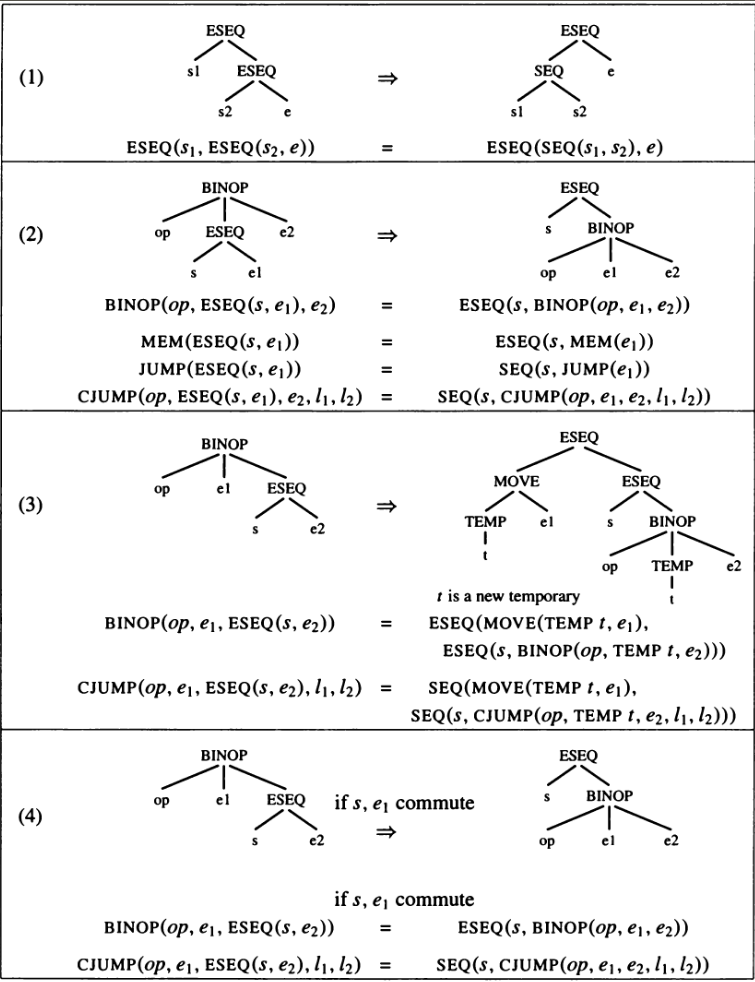
\includegraphics{assets/canon1.png}
\caption{ESEQ Removal}
\end{figure}

The transformation is done in three stages: First, a tree is rewritten
into a list of canonical trees without
\mintinline[breaklines=true, tabsize=2, breaksymbolleft=]{text}{SEQ} or
\mintinline[breaklines=true, tabsize=2, breaksymbolleft=]{text}{ESEQ}
nodes; then this list is grouped into a set of basic blocks, which
contain no internal jumps or labels; then the basic blocks are ordered
into a set of traces in which every
\mintinline[breaklines=true, tabsize=2, breaksymbolleft=]{text}{CJUMP}
is immediately followed by its false label.

\hypertarget{signature}{%
\subsection{Signature}\label{signature}}

\begin{minted}[breaklines=true, tabsize=2, breaksymbolleft=]{sml}
signature CANON = 
sig
  val linearize : Tree.stm -> Tree.stm list
    (* 
      From an arbitrary Tree statement, produce a list of cleaned trees satisfying the following properties:
      1.  No SEQ's or ESEQ's
      2.  The parent of every CALL is an EXP(..) or a MOVE(TEMP t,..)
    *)

  val basicBlocks : Tree.stm list -> (Tree.stm list list * Tree.label)
    (* 
      From a list of cleaned trees, produce a list of basic blocks satisfying the following properties:
      1. and 2. as above;
      3.  Every block begins with a LABEL;
      4.  A LABEL appears only at the beginning of a block;
      5.  Any JUMP or CJUMP is the last stm in a block;
      6.  Every block ends with a JUMP or CJUMP;
      Also produce the "label" to which control will be passed upon exit.
    *)

  val traceSchedule : Tree.stm list list * Tree.label -> Tree.stm list
    (* 
      From a list of basic blocks satisfying properties 1-6, along with an "exit" label, produce a list of stms such that:
      1. and 2. as above;
      7. Every CJUMP(_,t,f) is immediately followed by LABEL f. The blocks are reordered to satisfy property 7; also in this reordering as many JUMP(T.NAME(lab)) statements as possible are eliminated by falling through into T.LABEL(lab).
    *)
end
\end{minted}

\end{document}
